\chapter{Metodologia}
\label{cap-metodologia}
Este capítulo aborda sobre tudo que compõe a metodologia de pesquisa e construção
da solução, contendo os procedimentos e técnicas utilizados no trabalho, a fim de
explicar como o desenvolvimento foi realizado para atingir os seus objetivos,
servindo como base para a sua reprodução em trabalhos futuros.

A pesquisa é fundamentada e metodologicamente construída objetivando a resolução
ou o esclarecimento de um problema. O problema é o ponto de partida da pesquisa.
Da sua formulação dependerá o desenvolvimento da sua pesquisa
\cite{moresi2003metodologia}, neste trabalho a questão problema a ser resolvida é:

\begin{center}
  \textit{
  Como implantar aplicações web em sistema Debian GNU/Linux de forma automatizada e
  e segura?
}
\end{center}

Dado a questão problema, e o objetivo da implantação automatizada
de aplicações em sistema Debian GNU/Linux, este trabalho consiste em contribuir
com a construção de uma solução de engenharia de software que resolva a questão
problema, essa construção será feita a partir dos conhecimentos adquiridos durante
o curso de engenharia de software, além disso a solução proposta deverá passar
por uma validação dos resultados, utilizando uma validação baseada na observação
da execução da solução em exemplos de uso, onde cada exemplo de uso terá novos
desafios para testar a solução proposta. Essa validação tem seus procedimentos
definidos na seção \ref{subsection:validacao} e as definições dos exemplos de uso
estão na seção \ref{subsection:exemplos}.

Inicialmente será feito uma pesquisa nos trabalhos relacionados para entender
melhor o problema, e para guiar essa pesquisa será utilizado a definição de uma
metodologia de pesquisa. De acordo com\cite{gerhardt2009metodos} existem diferentes
tipos de pesquisa, elas podem ser classificados quanto sua abordagem, sua natureza,
seus objetivos e seus procedimentos. Por isso é importante selecionar a modalidade
de pesquisa adequada ao objeto de pesquisa.

Assim a pesquisa inicial será classificada quanto à natureza como pesquisa aplicada
pois tem como objetivo gerar conhecimentos para aplicação prática\cite{gerhardt2009metodos},
relacionada a aplicações que auxiliam na implantação automatizada de software.
Quanto a abordagem, a pesquisa é classificada como qualitativa, para buscar entender
o uso da automação da implantação de aplicações, exprimindo o que convém
a ser feito.

Quanto aos objetivos, esta pesquisa é classificada como pesquisa descritiva, que
exige do investigador uma série de informações sobre o que deseja pesquisar
\cite{trivinos1987introduccao}. Quanto aos procedimentos técnicos, serão utilizados
neste trabalho a pesquisa bibliográfica baseada no levantamento de referências
teóricas em livros e artigos científicos, permitindo conhecer os trabalhos
relacionados. A figura\ref{fig:metodologia1} apresenta de forma resumida a
classificação da pesquisa:

\begin{figure}[h]
  \centering
  \caption{Resumo da classificação de pesquisa}
  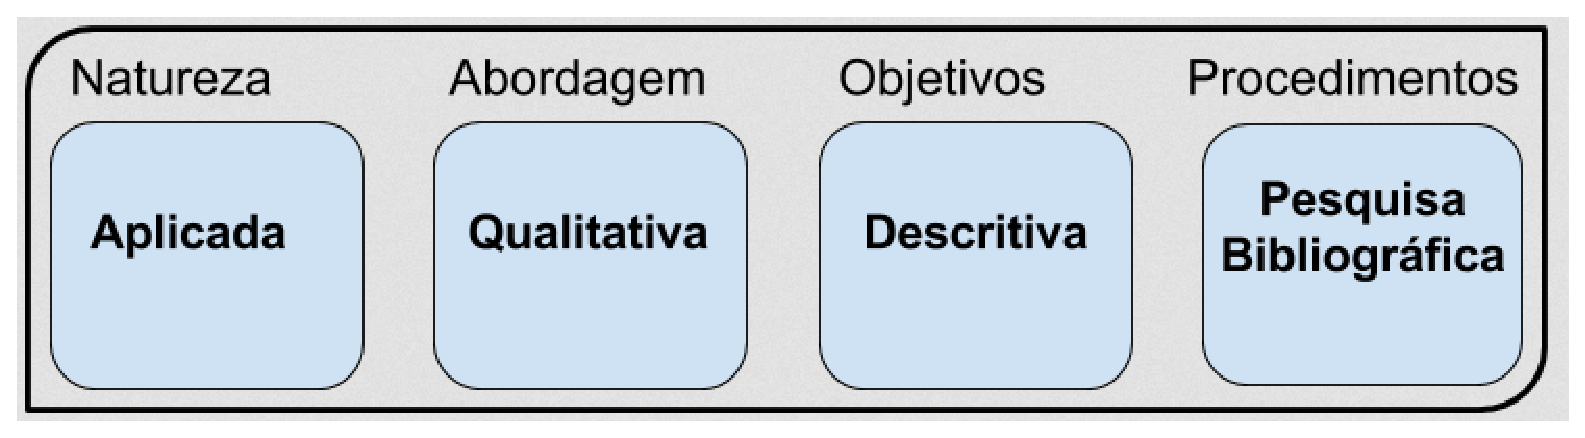
\includegraphics[width=1.0\textwidth]
      {figuras/met1.eps}
      Fonte: Elaborada pelo autor.
\label{fig:metodologia1}
\end{figure}

A partir da metodologia definida é possível encontrar os trabalhos relacionados
pela pesquisa científica, os trabalhos encontrados também serão de insumo para iniciar
a construção da solução a partir da análise dos resultados encontrados,
as próximas seções tratam dos trabalhos relacionados encontrados e dos métodos e
procedimentos para construção da solução, além da validação da solução.

\section{Trabalhos Relacionados}
\label{section:trabalhos_relacionados}
Para responder a questão problema primeiramente deve ser feito um levantamento
de trabalhos relacionados, para entender melhor como a automação da implantação
de software está sendo utilizada como solução na academia e nas empresas, e
quais são os procedimentos e técnicas utilizados.

Para entender o que acontece na comunidade da computação em relação a implantação
automatizada de aplicações, foi feito uma busca de alguns trabalhos relacionados, o primeiro
trabalho relacionado é um trabalho acadêmico feito por\cite{leo2014} no qual foi
desenvolvido um sistema de middleware chamado CHOReOS Enactment Engine que é um
sistema que possibilita a implantação distribuída e automatizada de composições
de serviços web em uma estrutura virtualizada, no qual opera no modelo
computacional conhecido como plataforma como serviço, comparando esse sistema
com abordagens ad-hoc de implantação levando em consideração a escalabilidade
em relação ao tempo de implantação das composições dos serviços.

Existem também ferramentas disponíveis no mercado que também trazem a proposta
de automação de instalação de aplicações alguns exemplos são:\cite{bitnami}
BitNami que é uma biblioteca de aplicativos de servidor populares e ambientes de
desenvolvimento que pode ser instalado com um clique. Ele automatiza todo o
processo de compilar e configurar os aplicativos e todas as suas dependências
(bibliotecas de terceiros, linguagem de programação, bases de dados) para que o
usuário comum não se preocupe com questões mais técnicas. Também temos o\cite{sandstormio}
Sandstorm é uma plataforma de código aberto para servidores
pessoais. Sandstorm permite que você execute o seu próprio servidor e instalar
facilmente as aplicações em que dão suporte, e por fim a ferramenta\cite{juju}
Juju que lhe permite implementar, configurar, gerenciar, manter e serviços de forma
rápida e eficiente automatizando a instalação e configuração de aplicações na nuvem.

O estudo dessas aplicações serve como base para entender como são feitas as
arquiteturas que são utilizadas pela comunidade da computação, por exemplo o JuJu
utiliza uma abstração conhecida como charm, que é basicamente um código que pode ser
escrito em várias linguagens, e esse código define um serviço, como por exemplo,
instale a aplicação de banco de dados ou instale a aplicação wordpress. Um charm
contém toda a lógica de que você precisa para implementar e integrar uma aplicação,
contendo todo o processo de download de ferramentas, instalação e configuração de
aplicações, podendo ser por provisionadores como chef, puppet ou docker\cite{juju},
é possível reaproveitar os charms feitos pela comunidade do JuJu assim
reaproveitando os charms prontos ou não precisando escrever um charm do zero.

Já bitnami já trás as aplicações
prontas pra uso, assim o usuário interage no formato clique para instalar, porém
o usuário só tem a disposição as aplicações disponibilizadas pelo bitnami, isso
também é a forma em que o sandstorm.io trabalha, com a diferença de que o standstorm é
software livre. Já o trabalho feito por\cite{leo2014} é voltado para serviços web
de grande escala, com foco em implantação de aplicações na nuvem e escalar infraestrutura, utilizando o middleware
construído em seu trabalho, assim podendo gerenciar ambientes de computação em nuvem
como Amazon EC2 e Openstack, sua engine utiliza o chef solo como seu agente de configuração.

Com esse levantamento vemos que existem algumas soluções que seguem a mesma
linha do que este trabalho pretende atingir como objetivo, servindo como motivação
para o seu desenvolvimento. Assim visto que a utilização do empacotamento
como técnica de implantação, traz inúmeras vantagens no processo de implantação
de aplicações como citado no capítulo\ref{cap-introducao}, tendo o levantamento
dos trabalhos relacionados e a questão de pesquisa como insumo, justifica-se a
construção de uma solução de engenharia de software para implantação automatizada
de aplicações em sistemas Debian GNU/Linux.

\section{Construção da solução}
\label{section:construcao}

A engenharia de software é a área da computação que busca evoluir de forma contínua
todos os aspectos da produção de um software, procurando sempre a garantia da
qualidade do produto desenvolvido. Segundo\cite{pressman2011engenharia}, a engenharia
de software é composta por um conjunto de três elementos fundamentais:

\begin{itemize}
  \item \textbf{Métodos:} Como fazer a implementação do software, com modelos,
  especificações e critérios para qualidade.
  \item \textbf{Ferramentas:} Objetivo de apoio automatizado para auxiliar as atividades
  de engenharia de software.
  \item \textbf{Processos:} Definem a sequência de práticas que serão utilizadas no
  desenvolvimento.
\end{itemize}

Seguindo esses três elementos, é possível definir como será construído a solução.
Primeiramente, é necessário definir o método de desenvolvimento de software, o
método que será seguido para desenvolvimento de software é o método ágil chamado
programação extrema (XP), de acordo com\cite{796139} essa metodologia contém um
conjunto de práticas que auxiliam um engenheiro de software. Dentro das práticas
que estão em\cite{796139} foram escolhidas as que poderiam ser aplicadas no
contexto deste trabalho, e são elas:

\begin{itemize}
  \item \textbf{Pequenas versões:} Implementar pequenas versões para conseguir
  um feedback mais rápido, atualizando o software frequentemente.
  \item \textbf{Design simples:} O código desenvolvido deve ser o mais simples possível,
  facilitando o entendimento de outros desenvolvedores que venham a ler o código.
  Além disso o código desenvolvido não deve fazer mais do que foi definido como
  requisito do software.
  \item \textbf{Refatoração:} O código pode ser reestruturado e seu comportamento
  continuar o mesmo, é muito utilizado para remover duplicações de código, deixar
  o código mais simples e fácil de dar manutenção.
  \item \textbf{Programação em pares:} A produção do software deve ser feita por duas
  pessoas utilizando a mesma máquina, no contexto deste trabalho a programação
  em pares será feita com o orientando fazendo par com o orientador ou coorientador,
  sempre que possível.
  \item \textbf{Revisão de código:} Todo o código produzido deverá ser revisado
  por um programador mais experiente, para que assim evite que erros sejam
  adicionados no código, e que o novo código adicionado seja bom o suficiente
  e possa ser aceito, no contexto deste trabalho a revisão de código será
  feita pelo co-orientador.
\end{itemize}

O ciclo de desenvolvimento terá iterações com duração de uma semana, ou seja,
o planejamento das atividades deverá levar em consideração que a
estimativa de todas as atividades escolhidas para a iteração não poderá
ultrapassar a duração de uma semana, dentro dessa semana além do desenvolvimento
das funcionalidades também deve levar em consideração a revisão de código, já que
nela pode acarretar pequenas correções que serão necessárias antes do código novo
ser incorporado, e isso pode levar algum tempo para ser feito, por isso a importância
de não deixar a revisão de código para o último dia da interação. A figura\ref{fig:def}
resume o ciclo de desenvolvimento:

\begin{figure}[h]
  \centering
  \caption{Resumo do ciclo de desenvolvimento}
  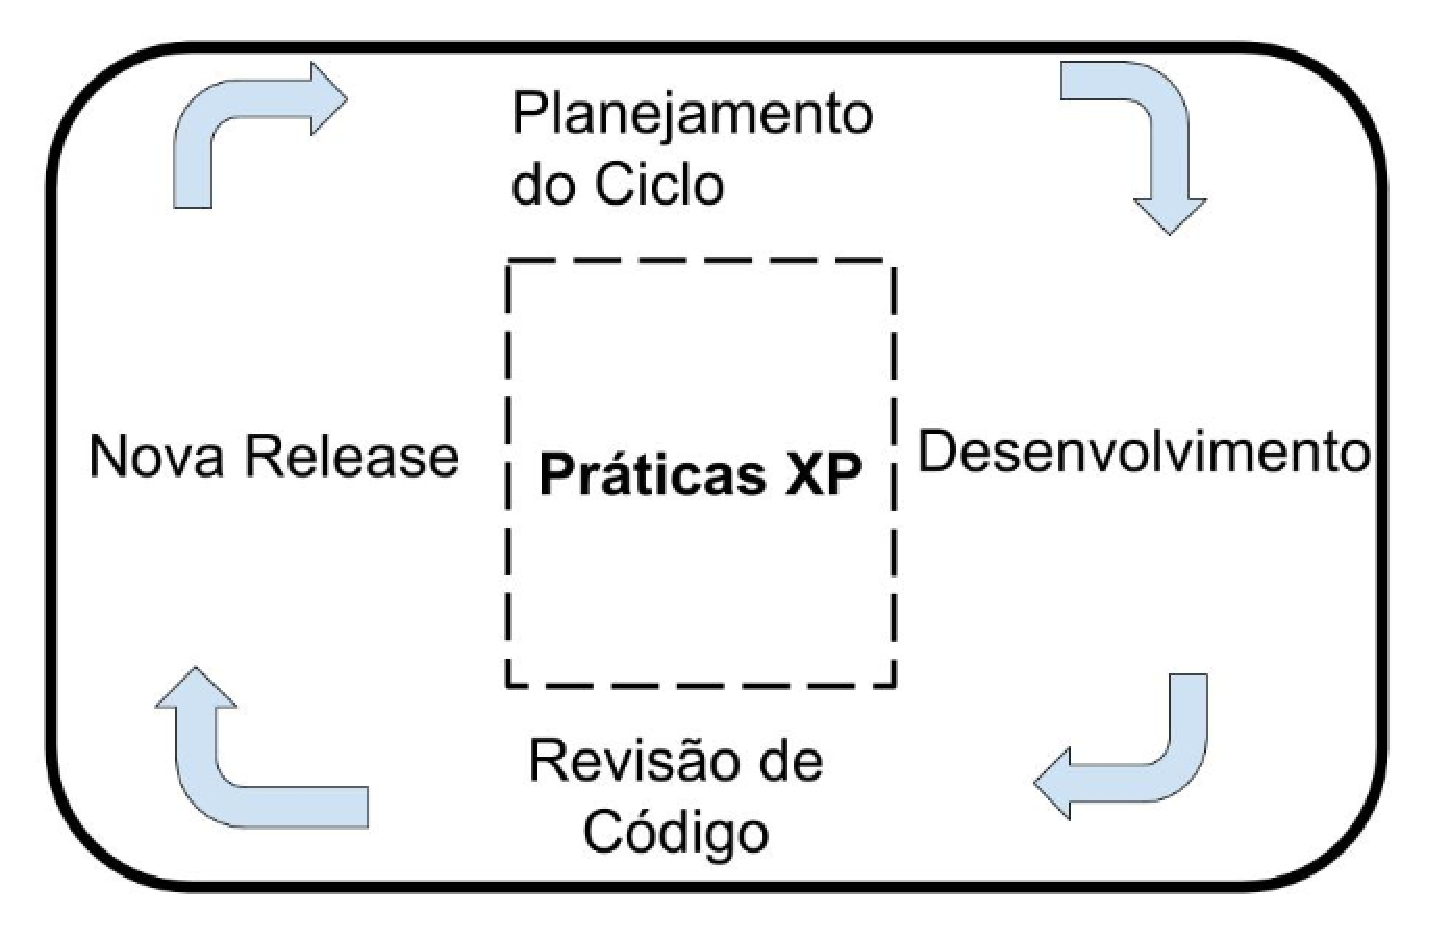
\includegraphics[width=1.0\textwidth]
      {figuras/desenvolvimento.eps}
  Fonte: Elaborada pelo autor.
\label{fig:def}
\end{figure}

As ferramentas de apoio ao desenvolvimento de software são importantes para a
organização do trabalho, auxiliando nas atividades típicas dentro de um projeto
de engenharia de software. Algumas ferramentas são importantes pois tornam mais fácil
a execução de algumas atividades, como por exemplo: o controle de versão do software,
ferramenta para documentação do software e ferramenta para gerenciar as tarefas.
Os critérios para escolha das ferramentas são:

\begin{itemize}
  \item \textbf{Forge para sistema de controle de versão git:} Uma ferramenta que
  possa gerenciar diversas versões do desenvolvimento do código fonte utilizando
  o sistema de controle de versão git, que seja de preferência um software livre
  ou que não cobre o serviço de hospedagem. Algumas ferramentas disponíveis para
  isso são github, gitlab e bitbucket.
  \item \textbf{Ferramenta para documentação de código:} Uma ferramenta que possa
  documentar o projeto, os forges como gitlab e github possuem uma wiki já disponível
  para o projeto.
  \item \textbf{Ferramenta de gerenciamento de tarefas:} Uma ferramenta que possa
  gerenciar as tarefas que serão executadas, que estão em execução ou que vão ser executadas
  durante o desenvolvimento do projeto. Essa ferramenta será importante para a
  organização do trabalho, dando visibilidade do trabalho que está sendo realizado.
  \item \textbf{Ferramenta de comunicação:} A ferramenta de comunicação será
  importante para tirar dúvidas rápidas em relação a dificuldades e desafios, as
  comunidades de software livre costumam usar listas de e-mail e canais no IRC
  para a comunicação de seus desenvolvedores e usuários.
\end{itemize}

Por fim é necessário definir a sequência de práticas e atividades que serão
utilizadas no desenvolvimento, definindo arquitetura básica para a solução de
implantação automatizada de aplicações. Portanto é preciso definir alguns
procedimentos importantes para a construção da arquitetura inicial considerando
o processo de implantação de software visto no capítulo\ref{cap-introducao}
e a referência dos trabalhos relacionados. Os procedimentos são os seguintes:

\begin{itemize}
  \item  \textbf{Definir as fases e os procedimentos para implantação automatizada:}
   Definir quais são etapas da implantação, definir a ordem necessária para a execução de
  cada fase da implantação, dado a importância de definir as fases que compõem o processo de
  implantação e de acordo com\cite{omg2006}.
  \item  \textbf{Definir os procedimentos de segurança na implantação:} Definir
  quais são os procedimentos de segurança e automatizar os que forem possíveis
  de serem aplicados dentro do contexto da arquitetura proposta. Um exemplo
  é a configuração das aplicações sempre usarem protocolos seguros, como o https
  que possui uma camada adicional de segurança que utilizando o protocolo ssl/tls.
\end{itemize}

Dentro da implantação automatizada de software Debian GNU/Linux temos várias
possibilidades, porém neste trabalho alguns aspectos que deverão ser levados em
consideração, esses aspectos serão importantes para guiar a construção da solução.

\begin{itemize}
  \item  \textbf{A1:} Uso dos aspectos de segurança na implantação de aplicações web.
  \item  \textbf{A2:} Uso da implantação automatizada de múltiplas instâncias de
   aplicações no mesmo servidor.
  \item  \textbf{A4:} Uso de aplicações que são empacotadas no debian.
  \item  \textbf{A5:} Uso de boas práticas de implantação de software.
\end{itemize}

Com essa base definida o próximo passo é definir quais serão as ferramentas
escolhidas que possibilitem a construção da solução, além de uma ferramenta
que possibilite a criação de um ambiente de desenvolvimento, já que dado o
contexto de implantação de software, é importante possuir um ambiente flexível
para testar facilmente a instalação e configuração das aplicações,
podendo facilmente reinicializar esse ambiente de forma que ele fique limpo sem
resquícios da instalação anterior.

\subsection{Ferramentas}

Para automatizar a instalação das aplicações é necessário escolher as ferramentas
que permitirão otimizar a instalação de aplicações, de acordo com \cite{6265084}
um grande facilitador do DevOps são as ferramentas de gerenciamento de configuração.
Tais ferramentas permitem controlar e automatizar a configuração de todos os
elementos que compõem uma aplicação, são elas: softwares previamente instalados,
usuários, serviços em execução, arquivos de configuração, tarefas programadas,
configurações de rede, armazenamento, monitoramento e segurança. Um exemplo citado
no trabalho feito em \cite{leo2014} no qual ele utiliza a ferramenta chef para
essas tarefas.

Neste trabalho, de acordo com a motivação da contribuição em software livre
e a participação do google summer of code como dito na seção de motivação
\ref{sec:motivacao}, e todo o contexto definido na seção \ref{section:construcao},
a ferramenta para apoio a implantação de software escolhida
será a ferramenta shak, a ferramenta shak é basicamente composta de:

\begin{itemize}
  \item  \textbf{Livro de Receitas Chef:} Shak contém alguns livros de receitas
  para poder organizar a instalação de cada componente, como por, exemplo um livro
  de receitas para cada aplicação que for instalada.
  \item  \textbf{Código Ruby} A arquitetura do Shak foi desenvolvida na linguagem
  ruby, com programação orientado a objetos.
  \item  \textbf{Servidor Web} O Shak utiliza o software livre Nginx, que é
  servidor HTTP de alto desempenho\cite{nginx}.
  \item  \textbf{Pacotes Debian} O Shak utiliza pacotes incluídos na distribuição
  oficial do Debian.
  \item  \textbf{Gems} O shak também utiliza algumas gems para seu funcionamento,
  uma gem nada mais é do que uma biblioteca, que provê um formato padrão para
  a distribuição de programas Ruby\cite{gem}.
  \item  \textbf{Código Shellscript} O shak também utiliza algumas gems para seu funcionamento,
  uma gem nada mais é do que uma biblioteca, que provê um formato padrão para
  a distribuição de programas Ruby\cite{gem}.
\end{itemize}

As ferramentas escolhidas para o apoio ao desenvolvimento foram:
\begin{itemize}
  \item \textbf{Forge Git:} O Gitlab foi forge escolhido para o armazenar o
  repositório git, é semelhante ao github, porém é software livre, distribuído pela
  licensa mit\cite{gitlab}.
  \item \textbf{Documentação de Código:} Toda documentação será disponibilizada
  na wiki do projeto no gitlab.
  \item \textbf{Gerenciamento de Tarefas:} O gerenciamento de tarefas também será
  feito pelo projeto do gitlab, onde é possível criar atividades para serem feitas
  e criar marcos podendo adicionar as atividades a esses marcos. Como o ciclo de
  desenvolvimento será de uma semana, serão criados marcos para cada semana e atividades
  agrupadas em cada marco.
  \item \textbf{Comunicação:} A comunicação será feita via IRC, é uma ferramenta
  de comunicação no formato de chat com canais e usuários dentro dos canais,
  apesar de ser uma ferramenta antiga ainda é muito usada pelas comunidades de software
  livre e grandes empresas como facebook\cite{artigofacebook}.
\end{itemize}

Por fim a ferramenta escolhida para gerenciar o ambiente de desenvolvimento e
ambiente de testes é a ferramenta Vagrant que é uma ferramenta que torna mais fácil
a configuração de ambientes de desenvolvimento, sendo eles reprodutíveis e
portáteis para ajudar a maximizar a produtividade e a flexibilidade necessária
de construir e destruir ambientes virtuais.\cite{vagrant}

Com a base de ferramentas definidas agora é necessário definir quais são as
aplicações que servirão como caso de testes para a implementação da solução. Elas
serão importantes pois a partir delas e de suas necessidades que serão feitos as
validações da solução e seus refinamentos. Após a escolha das aplicações que
servirão como exemplos de uso e os ambientes definidos é que será possível
iniciar o ciclo de desenvolvimento de software para a construção da solução.

\subsection{Validação da solução}
\label{subsection:validacao}

Para validar a arquitetura proposta no trabalho serão feitos exemplos de uso
com aplicações que possam servir para a execução da arquitetura construída, a
fim de refinar e evoluir a solução, a escolha desses exemplos de uso devem ser
feitas a partir de aplicações reais e conhecidas na comunidade de software livre.
 Para isso devem ser levados as seguintes características para a escolha das aplicações:

\begin{itemize}
  \item  \textbf{Aplicações empacotadas no debian:} Como o intuito do trabalho
  é realizar implantações múltiplas a partir de um pacote único, tais aplicações
  devem estar empacotadas e disponíveis para instalação nos servidores do debian.
  Isso impacta na escolha da ferramenta, visto que não será necessário ter o trabalho
  de empacotar aplicações que ainda não estão empacotadas no debian.
  \item  \textbf{Servidor web compatível:} As ferramentas escolhidas devem no
  mínimo possuir o servidor web compatível, por exemplo: as aplicações juntas
  devem possuir suporte para nginx ou apache ou similares.
  \item  \textbf{Aplicações com comunidades ativas:} Como estamos trabalhando
  com software livre, é importante que os softwares escolhidos possuem comunidades
  ativas, isso pode ajudar na resolução de possíveis problemas, logo aplicações
  em que sejam difíceis de comunicar com sua comunidade devem ser evitadas, e
  aplicações com a comunidade de desenvolvedores e usuários ativa devem ser priorizadas.
  E isso também pode ser um fator importante caso durante os testes sejam descobertos
  bugs ou melhorias dentro dessas ferramentas e tais bugs e melhorias possam ser
  reportados para a comunidade, ou até mesmo bugs solucionados e devolvidos aos mantenedores
  das ferramentas.
  \item  \textbf{Documentação do software:} A documentação do software também deve
  ser levado em consideração, principalmente a documentação da instalação e configuração
  dentro da ferramenta, ferramentas que não possuem documentação de instalação e
  configuração devem ser evitadas.
\end{itemize}

A partir dessas características definidas, é necessário encontrar os exemplos de uso
que possam servir para a execução da solução, todos as aplicações que servirão como
exemplos de uso devem pacotes incluídos na distribuição oficial do Debian.

\subsection{Exemplos de uso}
\label{subsection:exemplos}

Para encontrar as aplicações que possam se encaixar dentro desses parâmetros devemos
alguns exemplos de uso, com a finalidade de verificar se com tais métodos e
procedimentos atingirá o objetivo estabelecido. Para a escolha das aplicações que
serão utilizadas como exemplos de uso é necessário fazer uma busca nas aplicações
web que são empacotadas no debian e que possuem suporte a configuração de múltiplas
instâncias, essa busca deve levar em consideração também a documentação para realizar
tal configuração. Foram levantados algumas aplicações web empacotadas no debian da
seguinte forma:

\begin{center}
apt-cache search web | wc -l
\end{center}

O resultado obtido com pacotes que contenham a palavra web recebe o resultado de 3470
pacotes de diversas aplicações ou módulos de aplicações, como:
wordpress, owncloud, drupal, mailman, chromium, etc. Logo dentro dessa rápida busca
encontramos alguns pacotes de aplicações conhecidas, para facilitar a busca basta
aplicar para alguns nomes de aplicações conhecidos como:

\begin{center}
apt-cache search web | grep wordpress
\end{center}

Para avaliar se as aplicações possuem suporte a múltiplas instâncias é necessário
analisar a documentação das aplicações, as aplicações costumam disponibilizar a sua
documentação na sua página ou em uma wiki, também é possível checar a documentação
quando se instala uma aplicação nos arquivos de documentação da aplicação em
/usr/share/doc/ ou também pode-se utilizar os comandos:

\begin{center}
man nomeaplicação

info nomeaplicação
\end{center}

Analisando a documentação de algumas aplicações como wordpress, redmine,
owncloud, mailman, wikimédia, foram escolhidas as aplicações wordpress e owncloud por
atingirem completamente as características definidas anteriormente. Primeiro
foi feito uma análise da documentação dessas ferramentas para encontrar a
possibilidade da configuração de múltiplas instâncias no mesmo servidor, além
disso também foi visto se as aplicações tinham suporte ao servidor Nginx que é
o servidor utilizado pelo Shak, por fim as duas aplicações também foram escolhidas
pela grande comunidade de usuários ativa e as duas aplicações também possuírem
canais de IRC para tirar dúvidas com desenvolvedores e usuários.

Com as aplicações que serão exemplos de uso escolhidas a proposta de arquitetura
pode ser testada e validada, com o objetivo de criar múltiplas instâncias
no mesmo servidor de forma automatizada a partir de um pacote único, logo os
exemplos de uso também servirão para refinar e evoluir a arquitetura proposta.
Para realizar tais validações é importante que as instalações e configurações
sejam em um ambiente limpo, ou seja, os testes devem ser criados de preferência
em máquinas virtuais com a configuração conhecida como minimal, que contém
instalado apenas as aplicações necessárias para o funcionamento do sistema operacional.

A partir da execução dos exemplos de uso será possível a coleta de informações
necessárias para a validação da implantação correta das aplicações, essa
validação a princípio será feita a partir da execução da implantação e
verificação das funcionalidades da aplicação implantada, ou seja,
após a execução da implantação o testador deverá verificar o perfeito
funcionamento de algumas funcionalidades básicas da aplicação escolhida,
e principalmente verificar a implantação de várias instâncias da mesma
aplicação no mesmo servidor destino, observando o perfeito funcionamento de todas as
instâncias implantadas assim validando a implantação de múltiplas instâncias.
